\documentclass[11pt]{article}
\usepackage{tikz}

\usetikzlibrary{arrows}

\title{Bless, a pager\footnote{not like less}}
\author{void-}

\begin{document}
\maketitle
\section*{Overview}
\subsection*{Goal}
The Sender wishes to send a message to (page) the Receiver in real time. The
location of the Receiver should be private and the confidentiality, integrity,
and authenticity of the message should be preserved. The Sender must also be
approved to send messages to the Receiver, that is to say, not just anyone can
send a message to the Receiver. The system should work even if the Receiver is
behind a NAT.

\section*{An illustration}
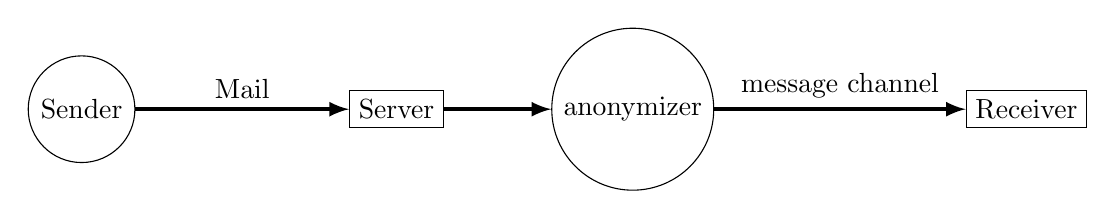
\begin{tikzpicture}
\node[draw, circle] at (0,0) (sender) {Sender};
\node[draw, rectangle] at (4,0) (server) {Server};
\node[draw, circle] at (7,0) (anonymizer) {anonymizer};
\node[draw, rectangle] at (12,0) (receiver) {Receiver};

\draw[arrows={-latex}, line width=.5mm]
  (sender) to node[above] {Mail} (server);
\draw[arrows={-latex}, line width=.5mm] (server) to (anonymizer);
\draw[arrows={-latex}, line width=.5mm]
  (anonymizer) to node[above] {message channel} (receiver);
\end{tikzpicture}

\pagebreak
\section*{Definitions}
\begin{itemize}
\item Sender \\
The entity that wishes to send a single message to the Receiver via the Server.
This can represent a number of authenticated individuals.
\item Server \\
The publicly routable server that authenticates messages from the Sender and
forwards them to the Receiver. Generally, the Server and the Receiver are
owned by the same individual.
\item Receiver \\
The entity that should receive a message from the Sender via the Server. The
Receiver's physical location in the world is consider private.
\item Message channel \\
The private communication channel established between the Server and Receiver.
\item Stale \\
When the message channel is stale, it means the Receiver has moved unbeknownst
to the Server. The Server will continue to attempt to communicate with the
Receiver using this channel even though the Receiver isn't listening.
\end{itemize}

\end{document}
